% !TEX root = main.tex

\section{Optimal control of Pitch/Travel without Feedback}
\subsection{1}
The continuous time system can be written as $\mathbf{\dot{x}} = \mathbf{A}_c\mathbf{x}+ \mathbf{B}_c\mathbf{u}$, with
\begin{subequations}
    \begin{align}
        \mathbf{x} &= \begin{bmatrix}
            \lambda\\
            r\\
            p\\
            \dot{p}
        \end{bmatrix}\\
        \mathbf{A}_c &= \begin{bmatrix}
            0 & 1 & 0 & 0\\
            0 & 0 & -K_2 & 0\\
            0 & 0 & 0 & 1\\
            0 & 0& -K_1K_{pp} & -K_1K_{pd}
        \end{bmatrix} \\
        \mathbf{B}_c &= \begin{bmatrix}
            0\\
            0\\
            0\\
            K_1K_{pp}
        \end{bmatrix}
    \end{align}
\end{subequations}

This is a model of the helicopter with pitch controller. The model inputs are set points for the pitch controller.

\subsection{2}
The system was discretized using forward Euler:
\begin{equation}
    \mathbf{\dot{x}} = \mathbf{A}_c\mathbf{x}_k + \mathbf{B}_c\mathbf{u}_k \approx \frac{\mathbf{x}_{k+1}-\mathbf{x}}{h}
\end{equation}

Rearranging, we get
\begin{equation}
    \mathbf{x}_{k+1} = (\mathbf{A}_ch + \mathbf{I})\mathbf{x}_k + h\mathbf{B}_c\mathbf{u}_k
\end{equation}

and we see that
\begin{subequations}
    \begin{align}
        \mathbf{A}_d &= \mathbf{A}_ch+\mathbf{I} \\
        \mathbf{B}_d &= h\mathbf{B}_c
    \end{align}

\end{subequations}

\begin{subequations}
    \begin{align}
        \mathbf{A_d} &= \begin{bmatrix}
        1 & h & 0 & 0\\
        0 & 1 & -hK_2 & 0\\
        0 & 0 & 1 & h\\
        0 & 0 & -hK_1K_{pp} & 1-hK_1K_{pd}
        \end{bmatrix}\\
        \mathbf{B_d} &= \begin{bmatrix}
        0\\
        0\\
        0\\
        hK_1K_{pp}
    \end{bmatrix}
    \end{align}
\end{subequations}

\subsection{3}
\begin{lstlisting}
    [z,lambda] = quadprog(Q,c,[],[], Aeq, beq, vlb, vub);
\end{lstlisting}

The optimal trajectory was calculated using quadprog, which takes a weight matrix Q, vector c (from the cost function $x^TQx + c^Tx$), inequality constraints matrices A, B, equality constraints Aeq, Beq and lower and upper bounds vlb, vub on the inputs, and returns a vector z with the optimal trajectory for all the states, along with a vector $\lambda$ containing the Lagrange multipliers at the solution.

\begin{lstlisting}
    Q1(1,1) = 1;
    ...
    P1 = 10;
    Q = 2*genq2(Q1,P1,N,M,mu);
    c = zeros(N*mx+M*mu,1);
    ...
    Aeq = gena2(A1,B1,N,mx,mu);
    beq = zeros(size(Aeq,1),1);
    ...
    [vlb,vub] = genbegr2(N,M,xl,xu,ul,uu);
\end{lstlisting}
The weight matrix Q was generated using the function genq2, and c is a vector of zeros. Aeq was generated using the function gena2, while beq is a vector of zeros. The constraints on the inputs were implemented using the given function genbegr2.

Finally, mx denotes the number of states, mu the number of inputs, N the time horizon for states and M the time horizon for inputs. For a more detailed description of the above functions, see Appendix X.\todo{make an actual reference}

The optimal input and optimal trajectory for the travel rate $\lambda$ are shown in the following plots.\todo{Add references}
%\clearpage %Let LaTeX handle this

\begin{figure}[h]
    \centering
    \makebox[\textwidth][c]{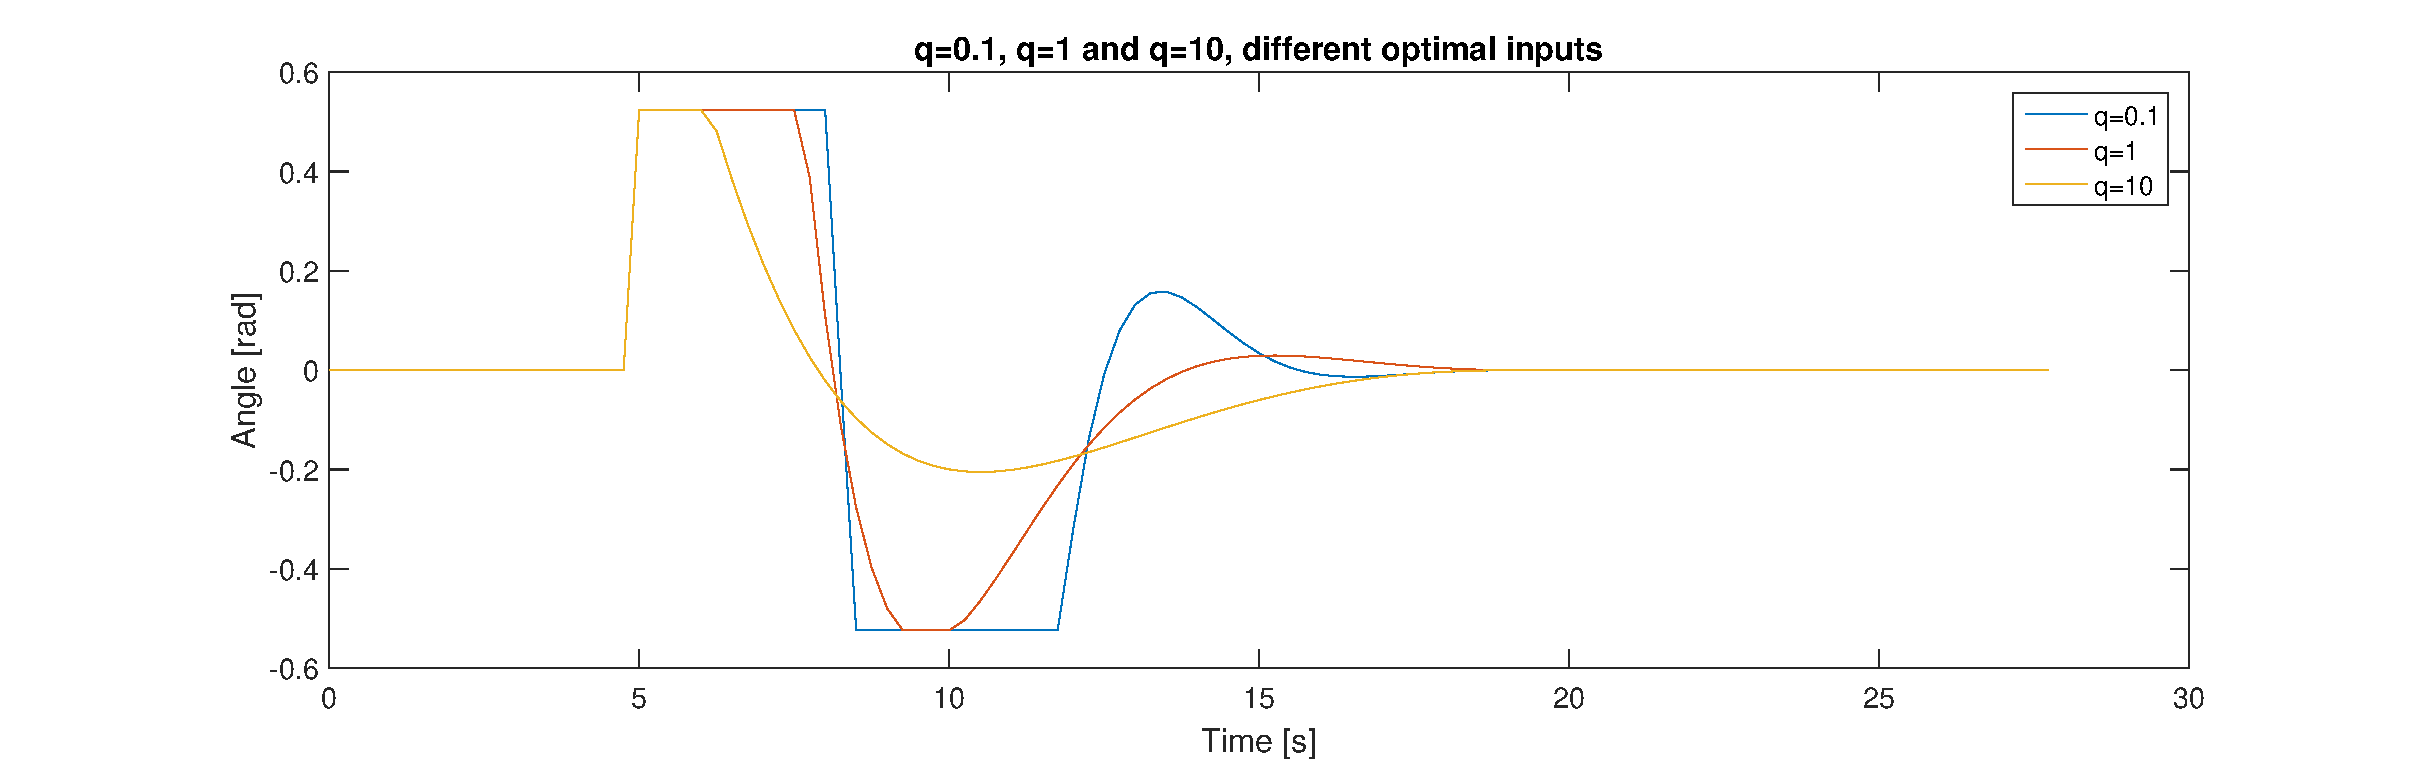
\includegraphics[width=1.2\textwidth]{task23_optimal_inputs.eps}}%
    \caption{Calculated optimal inputs}
    \label{fig:optimal_inputs}
\end{figure}

\begin{figure}[H]
    \centering
    \makebox[\textwidth][c]{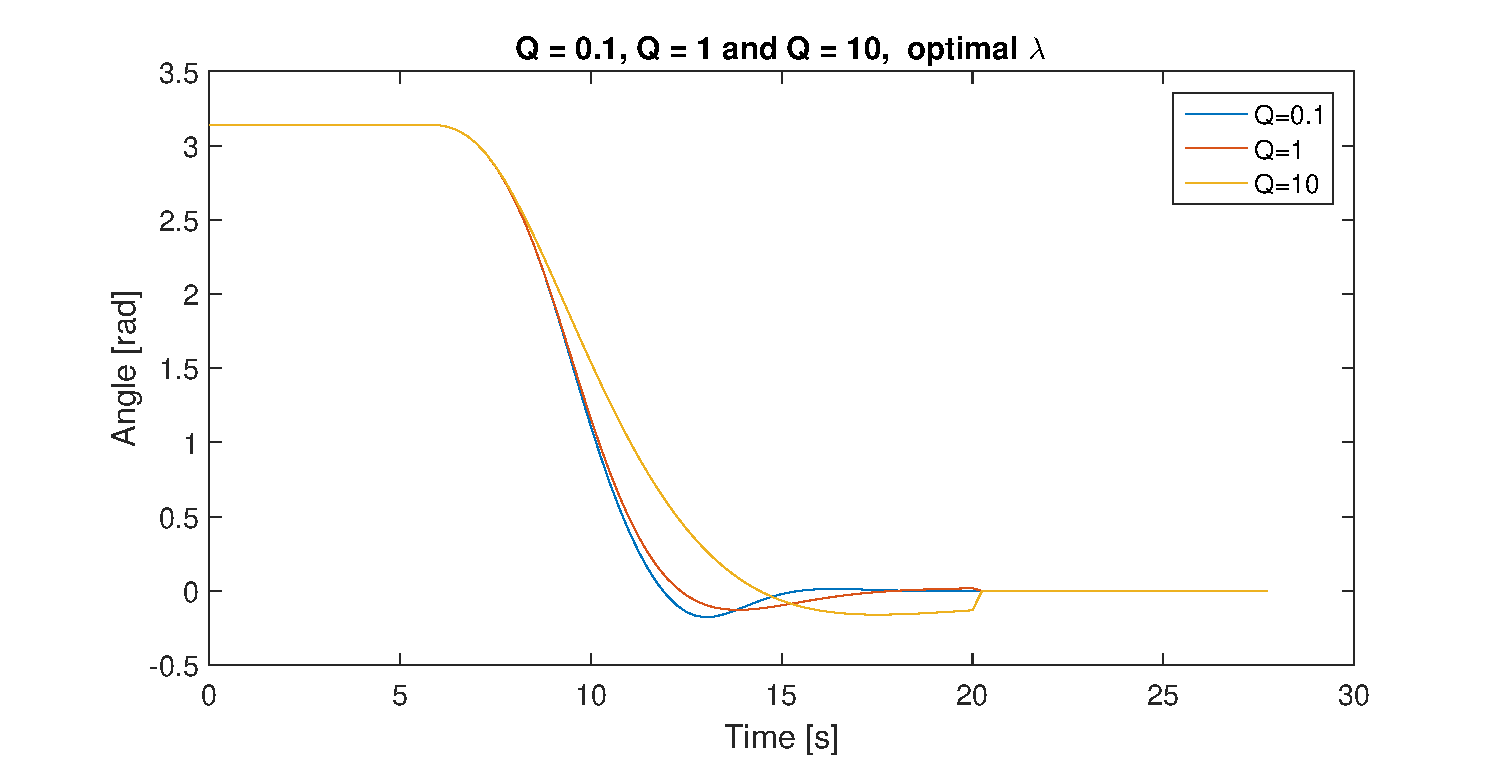
\includegraphics[width=1.2\textwidth]{optimal_lambda.eps}}
    \caption{Caption}
    \label{fig:optimal_lambda}
\end{figure}

The cost function \todo{insert cost function (15)} consists of two terms, $(\lambda_i - \lambda_f)^2$ and $qp_{ci}^2$. The first one aims to penalize deviation from the reference point $\lambda_f$, while the second one penalizes inputs $p_{ci}^2$. The relative cost of the two terms is set using the weight q. This can be seen in [\ref{fig:optimal_inputs}]; optimal input trajectories with larger Q are associated with a higher cost on the input, and are therefore more damped compared to optimal inputs with smaller Q. This is also reflected in [\ref{optimal_lambda}]; the optimal trajectory with the smallest weight is the fastest one, at the cost of some overshoot.

The smallest weight $Q=0.1$ gives the most aggressive control, but requires rapid changes in input, which might wear down the system over time. $Q=10$ on the other hand, seems rather slow. $Q=1$ seems like a good compromise; it is reasonably fast and not so hard on the actuators. In addition, [\ref{fig:optimal_lambda}] shows that it, at least in theory, gives the least amount of overshoot.

One downside of the cost function is that it does not include travel rate. So if the time horizon is not large enough, one might risk that it moves to the set point as fast as possible, without trying to stay there. In other words, it might have a high travel rate when it reaches the destination.

Another possible downside to the cost term $(\lambda_i - \lambda_f)^2$ could be that it does not take into account that $\lambda_i = \lambda_ i + 2\pi$, resulting in very poor pathing if exposed to a large perturbation. On the other hand, it might be desirable to actually perform one or multiple revolutions.
\todo{finner vi flere ulemper?}
\clearpage

\subsection{4}
The Simulink implementation is shown below. For the full Matlab code, see the Appendix.\todo{make actual reference}
\begin{figure}[H]
    \centering
    \makebox[\textwidth][c]{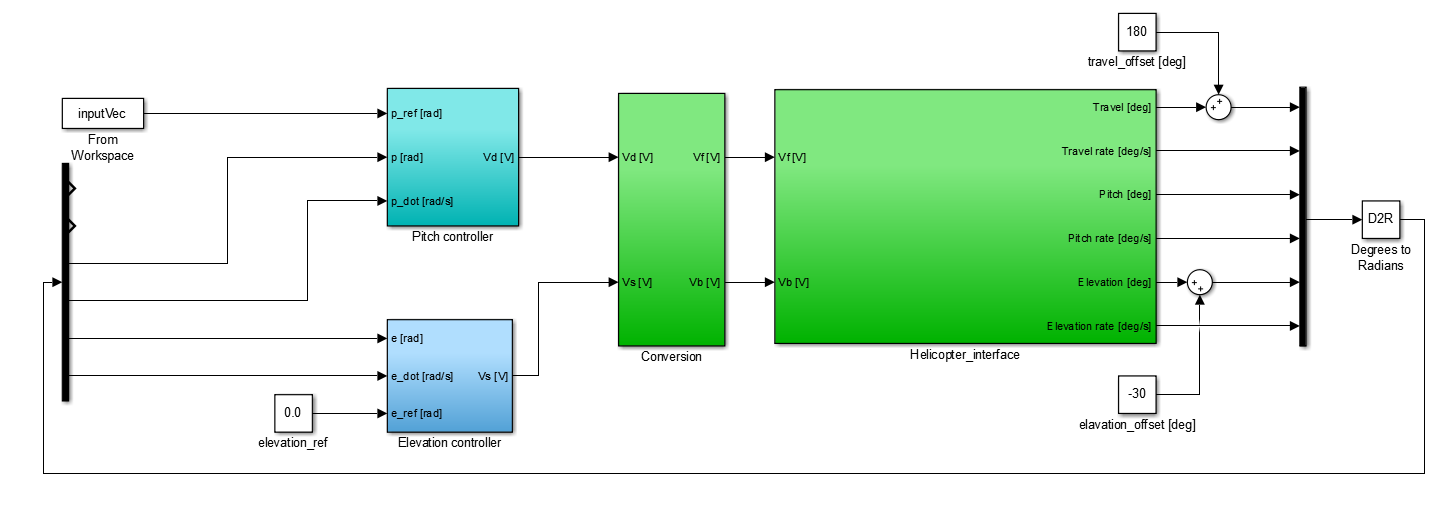
\includegraphics[width=1.2\textwidth]{E24_cropped.eps}}
    \caption{Caption}\todo{make actual caption}
    \label{fig:my_label}
\end{figure}

\begin{figure}
    \centering
    \makebox[\textwidth][c]{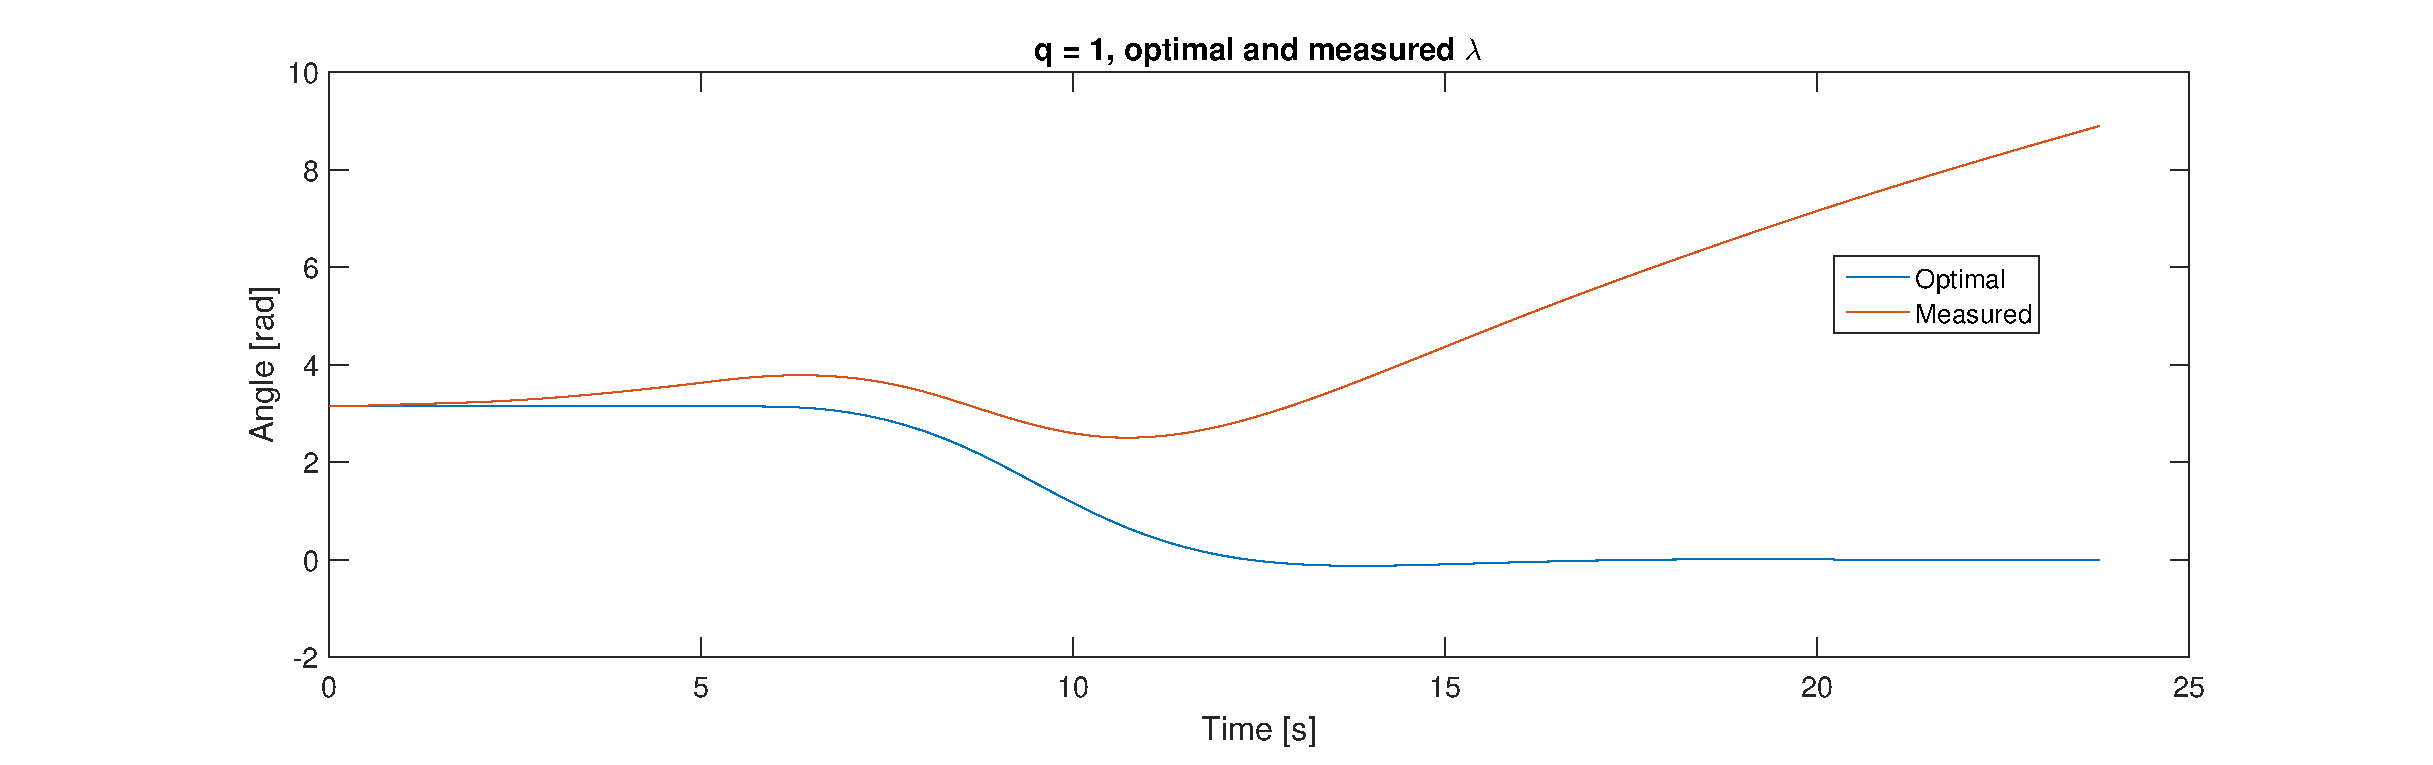
\includegraphics[width=1.2\textwidth]{optimal_and_measured_lambda.eps}}
    \caption{Caption}\todo{make actual caption}
    \label{fig:my_label}
\end{figure}

The helicopter does not end in the desired point $x_f$. There seems to be a constant error in travel rate or pitch. This is largely \todo{er det flere grunner?} because of model inaccuracies; discretization errors from using forward Euler and linearization errors, in addition to inherent model errors/simplifications. Also, the system is affected by noise (e.g. wind currents) as well as measurement errors.

\todo[inline]{Comment on helicopter drifting? UPDATE: Replace ? with !. Assumed in next part}

%\clearpage
